\chapter{Generic programming (genericity)}
\label{chap:genericity}

\lettrine[lines=2]{I}{n} natural language we say that something is generic when it can fit several purposes at once
while being decently efficient. For instance, a computer is a generic tool that allows one to write documents, access
emails, browse Internet, play video games, watch movies, read e-books etc. In programming, we will say that a tool is
generic when it can fit several purposes. For instance, the gcc compiler can compile several programming languages (C,
C++, Objective-C, Objective-C++, Fortran, Ada, D, Go, and BRIG (HSAIL)) as well as target several architectures (IA-32
(x86), x86--64, ARM, SPARC, etc.). Henceforth, we can say that gcc is a generic compiler. At this point it is important
to note that even though a tool is deemed generic, there is a scope on what the tool can do and what the tool cannot do.
A compiler despite supporting many languages and architectures, will not be able to make a phone call or a coffee. As
such it is important to note that genericity is an aspect that qualifies something. We will now studies the generic
aspects related to libraries and programming languages.

This thesis voluntary leaves out the generic aspect related to the target architecture. Indeed, being able to write
and/or generate code that is able to run on a large array of different hardware architecture is a field of research on
its own and is not the main focus of this thesis. It is also known as \emph{heterogeneous computing}. This field saw the
birth of its own standards (SYCL~\parencite{brown.2019.heterogeneous,wong.2019.heterogeneous}) and libraries solving
different problems, such as Halide~\parencite{ragankelley.2013.halide}, which provides its own DSL (Domain Specific
Language) to write code that will run on GPUs. In pure C++ there exists several high performance math library for linear
algebra, dense and sparse arithmetic which are optimized to produced very optimized code (vectorized instruction
support, parallel execution etc.). The most popular libraries are Eigen~\parencite{guennebaud.2010.eigen},
Blaze~\parencite{iglberger.2012_1.blaze,iglberger.2012_2.blaze,iglberger.2012.blaze},
Blitz++~\parencite{veldhuizen.2000.blitz,veldhuizen.1998.arrays} and
Armadillo~\parencite{sanderson.2016.armadillo,sanderson.2016.armadillo-art,sanderson.2018.armadillo-proc} leveraging
\emph{expression templates}~\parencite{veldhuizen.1995.expression} to achieve their goal. Also, we note that Eigen is
compatible with GPU source code~\parencite{guennebaud.2010.eigen-cuda} and can be used inside Cuda kernels. A Cuda
extension for Blaze was released recently~\parencite{penuchot.2019.blaze-cuda} and allow its use in GPU code as well.
Armadillo uses BLAS~\parencite{blackford.2002.blas} as underlying linear algebra routines which enables one to link
against the GPU-accelerated NVBLAS (NVidia)~\parencite{nvidia.2022.nvblas} or ACML-GPU
(AMD)~\parencite{amd.2013.acml-gpu} as drop-in replacement for BLAS to offload the work on GPU. All those libraries have
set performance as their main goal. They try to provide generic ways to solve issues related to parallelism and/or
vectorization while making use of expression templates for lazy computing (which will be seen
in~\cref{subsec:image.views.lazy.eval}). They do not aim to be able to handle as many input types as possible, however,
the lazy-computing techniques is used to generate new types on-the-fly. Henceforth, those libraries still need to embed
generic facilities to handle their own internal set of types. This thesis addresses genericity at the input level rather
than the target architecture level, henceforth, we will not address this topic here.

\paragraph{History} Genericity takes its root in~\citedate[year]{backus.1978.functional}
when~\citeauthor{backus.1978.functional} publishes his paper about functional
programming~\parencite{backus.1978.functional}. \citeauthor{backus.1978.functional} thinks that there exists five
computation forms with which one can build up all the rest of the computational infrastructure. Every piece of software,
for \citeauthor{backus.1978.functional}, is built from those five functional forms. Furthermore, the initial work of
\citeauthor{backus.1978.functional} does not use the possibility offered by mutations in his five computational forms.
These forms will lead to the birth of the functional programming paradigm (notably famous for its value immutability).
Stepanov, a mathematician, thinks that those forms are theorems. He also thinks that there is an infinite number of
theorem (as in mathematics) and that reducing their number to five for software programming is reductive. He publishes
in 1987~\parencite{stepanov.1987.higher} that one cannot ignore the mutability of states if one wants to achieve maximum
efficiency. Stepanov reasons about software programming by drawing a parallel with algebraic structures. Indeed, let us
consider the classical parallel computation model (map-reduce~\parencite{dean.2008.mapreduce}). In this model, being
able to reorder computation is a prerequisite in order to have a reduction that works. \emph{Reordering computation} can
be reworded as the \emph{associative property} of an algebraic structure, the monoid~\parencite{dean.2019.monoids} which
is a triplet consisting of a data structure, an associative binary operation and a neutral element. Stepanov thinks that
we extract those data structures and those laws/properties from software program the same way as we discover theorems
and axioms in mathematics. Software would then defined on top of algebraic structures, and it's the software
programmer's job to discover the data structures and laws that compose them.

This reflection leads to the publication of \citetitle{musser.1988.generic}~\parencite{musser.1988.generic} in which the
term \emph{Generic Programming} first appears. ``By generic programming, we mean the definition of algorithms and data
structures at an abstract or generic level, thereby accomplishing many related programming tasks simultaneously. The
central notion is that of generic algorithms, which are parametrized procedural
schemata~\parencite{goguen.1984.parametrized} that are completely independent of the underlying data representation and
are derived from concrete, efficient algorithms.''. This article lead to the genesis of the book
\citetitle{musser.1989.ada}~\parencite{musser.1989.ada} in which was published the first work about a generic library of
algorithms and data structures. Then Stepanov and Lee wrote the first version of the Standard Template
Library~\parencite{stepanov.1995.standard} in 1995 which is a carefully crafted library of basic algorithms to
manipulate algebraic structures (data structures) that is still an authority to this day. This standard template library
was then incorporated alongside the C++ language for the release of the first ISO standard of the language in 1998
\parencite{iso.1998.cpp}. That same year is published~\parencite{dehnert.1998.fundamentals}. This is the first place
where the term \emph{concept} appears as ``a set of axioms satisfied by a data type and a set of operations on it.''
This term is designed to include the complexity of an operation as part of an axiom in software programming. Also, it is
introduced to replace the previously used mathematical terms that could not carry the notion of complexity. It is also
the first place where the notion of \emph{regular} type appears: ``Since we wish to extend semantics as well as syntax
from built-in types to user types, we introduce the idea of regular type, which matches the built-in type semantics,
thereby making our user-defined types behave like built-in types as well.'' Efforts were made by
\citeauthor{gregor.2006.concepts-art} in~\parencite{gregor.2006.concepts-proc,gregor.2006.concepts-art} in 2006 to
introduce them into C++11~\parencite{iso.2011.cpp}, but it ultimately failed, and the feature was pulled off of the C++
standard~\parencite{seymour.2009.concepts}. This had major consequences on the language. Indeed, the standard body did
not publish a standard for 13 years, which is a long period in the information technologies area, leading to adoption of
more recent, more maintained/evolving languages by the industry. The standard body then decided to review its
publication process and has set a 3 years deadline in between each new standard release. Features must be ready in due
date before being merged into the next standard version or else they are delayed to the next standard version (3 years
later). The standard body decided that it will not wait for a feature to be ready to publish its next release.

Before publishing \citetitle{stepanov.2009.elements}~\parencite{stepanov.2009.elements}, Stepanov presented his view of
\emph{Generic programming} to Backus. Backus ``always knew that at some points he needed to figure out mutation into
functional programming and one view of generic programming is that generic programming is functional programming with a
well-defined way to handle mutation.'' Unfortunately Backus passed away before being able to write the forewords of
\citetitle{stepanov.2009.elements} book~\parencite{parent.2018.generic-programming}. The term \emph{generic programming}
never appears in his book because Stepanov thought he lost control over it. In practice, it has evolved into
metaprogramming, effectively associated to C++ template metaprogramming instead of being associated with the underlying
mathematics, algebraic structures, data structures and algorithms. This book introduces the \emph{require} clause on
algorithms in order to achieve constrained genericity.

In order to pursue the introduction of concepts into the C++ language, a workshop was held in 2012 and its summary was
published in \citetitle{sutton.2012.concepts}~\parencite{sutton.2012.concepts}. It is referred to as the \emph{Palo
  Alto} report, and it summarizes what design the committee wanted for concepts and what problem(s) it would
solve~\parencite{stroustrup.2012.concept}. Indeed, in \citetitle{stepanov.2009.elements} argues that just having
constrained template was already incredibly useful, and the STL could be described in terms of \emph{require} clauses.
This subset becomes known as ``concepts light'' and was enriched to become later what would be standardized in C++20.

Stepanov then published \citetitle{stepanov.2014.mathematics}~\parencite{stepanov.2014.mathematics} that traces the
history of algorithms and ties the history of mathematics with the history of generic programming. Indeed, Stepanov
already gave a lecture in 2003~\parencite{stepanov.2003.gcm} where he traces in particular the history of the algorithm
of gcd/gcm for 2500 years and explain how successive generation of mathematicians improved it by always looking for more
generic ways to solve the same problem. In essence, the book presents generic programming as an extension of the
evolution of mathematical algorithms over time. In this book, Stepanov also reclaims the term of \emph{generic
  programming} and differentiates it from template metaprogramming once and for all. Stepanov also states that ``Generic
programming is about abstracting and classifying algorithms and data structures. It gets its inspiration from
Knuth~\parencite{knuth.2014.art} and not from type theory. Its goal is the incremental construction of systematic
catalogs of useful, efficient and abstract algorithms and data structures. Such an undertaking is still a dream.''

Stepanov thought of STL as a starting point to a very large library of data structures and algorithms, written in a
generic form, that would all work together nicely. STL is intended to be an example of how industry should move forward
and work on building a large library of this form. Hopefully, this is the direction the C++ standard committee is going
toward.

\paragraph{Genericity within libraries} It is described by the cardinality of how many use-cases it can handle.
Libraries always provides their own data structures, to represent and to give a meaning to the data the user wants to
process, as well as algorithms to process those data and provide different type of results. A library will be then
labeled as \emph{generic}~\parencite{musser.1994.algorithm} when (i) its data structures allow the user to express
himself fully with no limitation and when (ii) its algorithm bank is large enough to do anything the user would want to
do with its data. In reality such a library does not exist and there are always limitations. Studying those limitations
and what reasons motivate them is the key to understand how to surpass them in the future, by developing new hardware
and/or software support for new features enabling more genericity.

\paragraph{Genericity within programming languages} It is described by the ability of the language to execute the same
code over a large amount of data structures~\parencite{dehnert.1998.fundamentals}, be they native (char, int, \ldots) or
user defined. It is nowadays primordial for a programming language to be able to do so. Indeed, in a world where
Information Technologies are everywhere, the amount of code written by software developers is staggering. And with it so
is the amount of bugs and security vulnerabilities. Being able to natively have a programming language that enables to
do \emph{more} by writing \emph{less} mathematically results in a reduced development and maintenance cost. Programming
languages offers many ways to achieve genericity which is dependent of the language intrinsic specificities: compiled or
interpreted, native or emulated, etc.

Before delving into the specifics of what genericity implies for libraries and programming languages, let us introduce
some vocabulary for the sake of comprehension. First is the notion of \emph{type}. A \emph{type} (or \emph{data type})
is an attribute of data which tells the compiler or interpreter how the programmer intends to use the data. Most
programming language support basic data types (also called primitive types) such as integer numbers, floating point
numbers, boolean and characters (ASCII, Unicode, etc.). This data attribute defines the operations that can be performed
on the data, the meaning of the data and the size of the data in memory (the data can then be stored on the heap, stack,
etc.). A data type provides a set of values from which an expression (\ie variable, function, etc.) may take those
values. Among programming language, we can distinguish those who are dynamically types and those that are statically
typed. Statically typed languages are those whose variables are declared holding a specific type. This variable cannot
hold data from another type in the scope it is declared. Statically typed programming languages are Ada, C, C++, Java,
Rust, Go, Scala. Dynamically types languages are those whose variables can be reassigned with a value of different type
from the one it was initially declared to hold. The variable type is then dynamically changed to fit the new value it is
holding. Dynamically typed programming languages are PHP, Python, JavaScript, Perl.

The consequence of being able to tell which type a variable is holding at all time (statically-typed language) is
two-fold. For the developer, it is easier to reason about code and to spot bugs. For the compiler, it is possible to
generate optimized binary code specific to this data type (vectorization, etc.). The consequence of being able to morph
the types a variable can hold at runtime is mainly to serve prototyping purpose. When tweaking a Jupyter notebook, it is
much appreciated not to be limited to a single type for each variable to be able to iterate on the prototype much
faster.

In image processing, an image \(Im\) is defined on a domain \(\mathcal{D}\) (which contains points) by the relation
\(\forall x \in \mathcal{D}, y = Im(x)\) where \(y\) is the value of the image \(Im\) for the point \(x\). This
definition always translates into a complex data structure when transposed into a programming language. This data
structure must be aware of the data buffer containing the image data as well as information about the size and
dimensions of the image. Furthermore, to add to the difficulty, the information needed to define precisely the data
structure is not always known when writing the source code. Indeed, a very simple use-case consists in reading an image
from a file to load it in memory. The file can contain an image of varying data type and the program should still work
properly. There are multiple approach to solve this issue, and we will address them in the
following~\cref{sec:gen.within.libraries} and~\cref{sec:gen.genericity.within.programming.languages}.



\section{Genericity within libraries}
\label{sec:gen.within.libraries}

Projecting the notion of genericity to Image Processing, we can deduce that we need two important aspects in order to be
generic. First, we need to decorrelate the data structures and its topology and underlying data from the algorithms.
Indeed, we want our algorithms to support as much data structures as possible. Second, many algorithms share the same
computational shape and can be factorized together.

\begin{figure}[htbp]
  \centering
  \begin{tabular}{cccc}
                                                                           & image 2D
                                                                           & graph    & mesh \\[5pt]
    input:                                                                 &
    \fbox{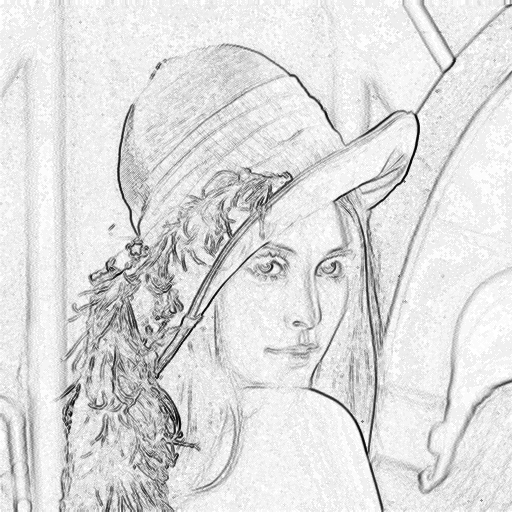
\includegraphics[width=.2\linewidth]{../figures/geninput-000b}}  &
    \fbox{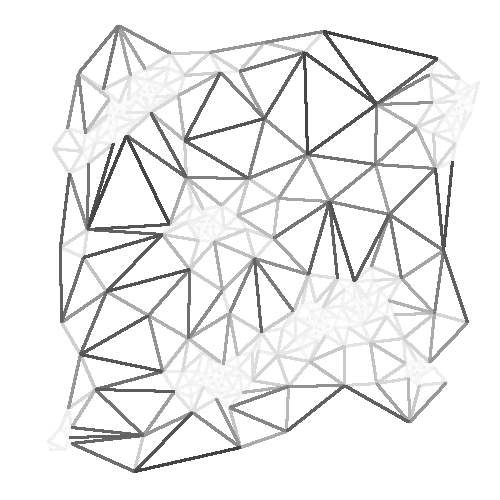
\includegraphics[width=.2\linewidth]{../figures/geninput-001b}}  &
    \fbox{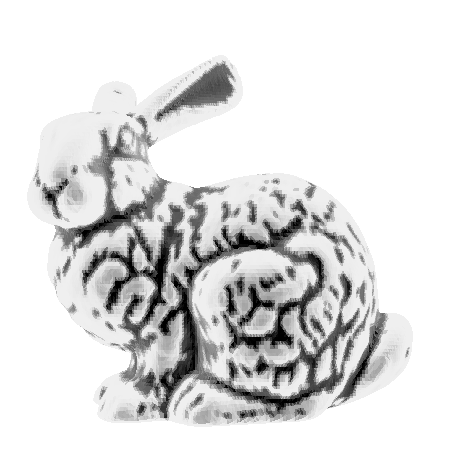
\includegraphics[width=.2\linewidth]{../figures/geninput-002b}}
    \\[5pt]
    %
    output:                                                                &
    \fbox{
\includegraphics[width=.2\linewidth]{../figures/genoutput-000}}  &
    \fbox{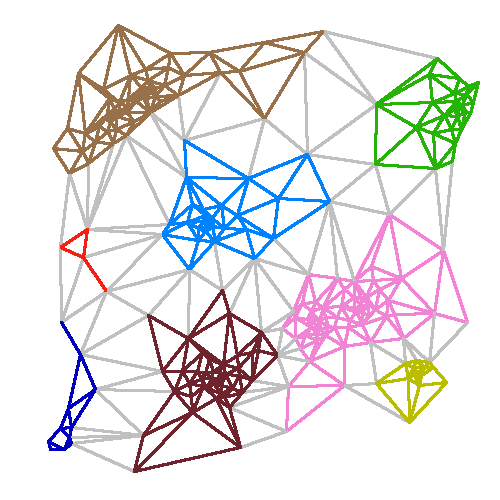
\includegraphics[width=.2\linewidth]{../figures/genoutput-001b}} &
    \fbox{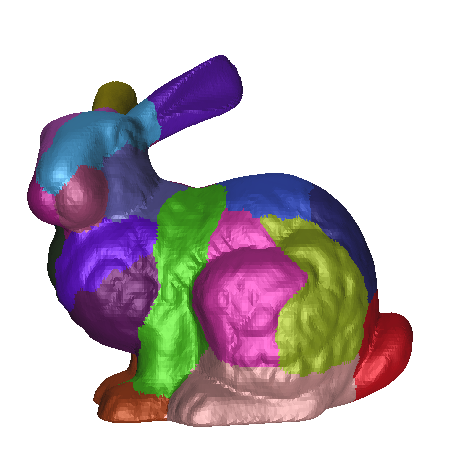
\includegraphics[width=.2\linewidth]{../figures/genoutput-002b}}
    \\
  \end{tabular}
  \bigskip

  \text{The same code run on all these inputs.}

  \caption{Watershed algorithm applied to three different image types.}
  \label{fig:type.vs.algo}
\end{figure}

Genericity can have two different meanings depending on the people you ask. For instance, some will argue that
genericity is high level and qualifies a tool which is ``generic enough'' to handle all of his use-cases. Others will
argue that genericity is about how a machine (code) is able to make tools, ``generic enough'' to make a lot different
tools. Neither is wrong. However, for the sake of comprehension we will use different words for each of these cases. A
tool generic enough to handle a lot of use-case will be called \emph{versatile}. Finally, for a tool whose aim is to
provide a programming framework to handle code of any use-case we will use \emph{generic}. In this thesis, genericity
will be about code. The~\cref{summary:fig:type.vs.algo} illustrates this result of the same generic watershed
implementation applied on an image 2D, a graph as well as a mesh.

In image processing, there are three main axes around which genericity is applying. The first axis is about the data type:
gray level or RGB color (8-bits, 10-bits), decimal (double) and so on. The second axis, is about the structure of the
image: a contiguous buffer (2D or 3D), a graph, a look-up table and so on. Finally, the third axis is about additional
data that can be fed to image processing algorithms: structuring element (disc, ball, square, cube), labels
(classification), maps, border information and so on. In the end, an image is just a point within this space of
possibilities, illustrated in~\cref{fig:gen.espaceSAV}. Nowadays, it is not reasonable to have specific code for every
existing possibility within this space. It is all the more true when one wants efficiency.

\begin{figure}[htbp]
  \centering
  \subfloat[]{\includestandalone[width=1.7in]{../figures/espaceSeI}}
  \hfil
  \subfloat[]{\includestandalone[width=1.7in]{../figures/espaceSAV}}
  \caption{The space of possible implementation of the \emph{dilation(image, se)} routine.\\
    The image axis shown in (a) is in-fact multidimensional and should be considered 2D as in (b).}
  \label{fig:gen.espaceSAV}
\end{figure}

Genericity is not new and was first introduced in 1988 by Musser et al.~\parencite{musser.1988.generic}. The main point
is to dissociate data structures and algorithms. The more your data structures and algorithms are tied together, the
less you will be generic and will fail to handle multiple data structures in the same algorithm. Further work has been
made about genericity in~\parencite{musser.1994.algorithm,dehnert.1998.fundamentals}. Those works highlight the notion
of abstraction to be able to turn an algorithm tied to a data structure into a generic algorithm. Notably
in~\parencite{stepanov.2009.elements}, Stepanov digs further and introduce the notion of \emph{Concepts}, which are
static requirements about the behavior of a type, by showing how to design a generic library and its algorithms. He
highlights the importance of having the algorithms driving the behavior requirements, and not the opposite. These works
are very suitable to be applied in the area of Image processing where we typically have a lot of algorithms (also called
operators) that are required to work on a lot of different data structures (also called image types).

The authors explain in~\parencite{roynard.2019.rrpr} how to capitalize on those works to turn a data-structure-specific
image processing algorithm into a generic algorithm. We also explain how \emph{concepts} can ease the implementation of
generic algorithms. This approach is implemented in a library~\parencite{carlinet.2018.pylena} which allows us to
provide a proof of concept over the feasibility of having generic image processing operators running on multiple image
types with near-native performance. Let us first explain briefly how we achieved this.

\subsection{Different approaches to get genericity}
\label{subsec:different.approaches}

First, let us consider the morphological \emph{dilation} that takes two inputs: an image and a flat structuring element
(SE). The set of some possible inputs is depicted in~\cref{fig:gen.espaceSAV}. Without genericity, with \(s\) the number
of image type, \(v\) the number of value type and \(k\) the number of structuring elements, one would have to write \(s
* v * k\) different \emph{dilation} routine.

There are several ways to reach a high level of genericity. First there are the \emph{code duplication} approach as well
as the \emph{generalization} approach. Finally, there is a way that consists in using expert, domain specific tools
specifically engineered for this purpose and build upon them: those tools usually make heavy usage of \emph{inclusion
  \& parametric polymorphism}, also known as template metaprogramming in C++, to provide the basic bricks the user needs
to build upon.

\paragraph{Code duplication approach} It consists in writing and optimizing the algorithm for a particular type in mind.
Then, each time a new type is introduced, all the algorithm must be rewritten for this specific type. Additionally, each
time a new algorithm is introduced, it must support all the existing types and thus be written multiple times. This
approach does not scale well when the complexity of algorithms grows, and the number of data types increases. Neither it
does allow the implementer to easily make use of optimization opportunities that can be offered by different data types
having a common property. This translates into heavy switch/case statement in the code as show in~\cref{code:gen.exhau}
that illustrate how the \emph{fill} algorithm needs to dispatch according to the input data type.

\begin{figure}[htbp]
  \centering
  \begin{minted}[linenos,xleftmargin=17pt,gobble=2]{cpp}
  // image types parametrized by their
  // underlying value type
  template <ValueType V> struct image2d<V> { /* ... */ };
  template <ValueType V> struct image_lut<V> {/* ... */};
  // ...
  void fill(any_image img, any_value v)
  {
    switch((img.structure_kind, img.value_kind))
    {
    case (BUFFER2D, UINT8):
      fill_img2d_uint8( (image2d<uint8>) img,
                        (uint8) any_value );
    // ...
    case (LUT, RGB8):
      fill_lut_rgb8( (image_lut<rgb8>) img,
                     (rgb8) any_value );
    }
  }
  \end{minted}
  \caption{Fill algorithm skeleton with a switch/case dispatcher to ensure completeness.}
  \label{code:gen.exhau}
\end{figure}

In addition, it is important to note that the completeness aspect is only illustrated regarding the data structure types
here. Indeed, the data structures are all already generic for their underlying data type (named \emph{ValueType} in the
code). When one write \texttt{image2d<uint8>} (l.10), it means \emph{2D-image whose pixels' have a single channel 8-bits
  value}. This approach enables one to write an algorithm at maximum efficiency for a particular data type, however one
can easily miss optimization opportunities if not knowledgeable enough too. This approach is best for early prototypes
and trying to find common behaviors pattern among algorithms, or common properties across different data types. No IP
library has chosen this approach due to the obvious maintenance issue induced.

\paragraph{Generalization approach} It consists in finding a common denominator to all the image types. Once designed,
this common denominator, also called super-type, can store information about all the supported image types by the
library. This super-type allows the library developer to write all the algorithms only once: for the super-type. The
processing pipeline will then consist in three steps. First convert the input image type into the super-type, second
process the super-type into the algorithm pipeline requested by the user, finally convert back the resulting image into
the specific image type the user is expecting. This approach offers the advantage of being maintainable. Adding a new
image type is just a matter of providing the two conversions facilities: to and from the super-type. Adding an algorithm
is also just a matter of writing it once for the super-type. This mechanism is shown in~\cref{code:gen.generalized}.
However, one must keep in mind that the conversion can be costly. Also, processing the super-type may induce a
significant performance trade-off while processing the original type would be much faster. Furthermore, it is not always
possible to find this common denominator when enumerating through some esoteric data types. Finally, the provided
interface (from the super-type) may allow the image to be used incorrectly, such as a \(2D\) image being processed into
video (\(3D+t\)) algorithm. Widely use libraries such as OpenCV~\parencite{bradski.2000.opencv},
Scikit-image~\parencite{vanderwalt.2014.skimage} use this technique to handle as many image types as possible. Another
library making use of this generalization technique in its implementation is CImg~\parencite{tschumperle.2012.cimg}.
CImg generalize its data type to a 4D image type templated by its underlying data type.

\begin{figure}[htbp]
  \centering
  \begin{minted}[gobble=2]{cpp}
  struct image4D { // generalized super-type
    // generalized underlying value-type
    // every value is converted to this one
    using value_type = std::array<double, 4>;
    /* ... */
   };
  // specific types w/ conversion routines
  struct image2D { image4D to(); void from(image4D); };
  struct image3D { image4D to(); void from(image4D); };
  // ...
  void fill(image4D img, const std::array<double, 4>& v) {
    for(auto p : img.pixels())
      p.val() = v;
  }
  \end{minted}
  \caption{Fill algorithm for a generalized super-type.}
  \label{code:gen.generalized}
\end{figure}

\paragraph{Inclusion \& Parametric polymorphism approach} They consist in extracting behavior patterns from algorithms
to group them into logical brick called \emph{concepts} (for static parametric polymorphism), or \emph{interface} (for
dynamic inclusion polymorphism). Each algorithm will require a set of behavior pattern that the inputs need to satisfy.
In C++, it can be done either by using inclusion polymorphism, or by using parametric
polymorphism~\parencite{gibbons.2007.datatype}, as shown in~\cref{code:gen.inclupoly}. In~\parencite{roynard.2019.rrpr},
we leverage a new C++20 feature (the concept) to show how it is possible to turn an algorithm, specific to an image
type, into a more abstract, generic one that does not induce any performance loss. This approach, especially applied to
image processing, will be seen more in-depth in~\cref{chap:image.algorithms.taxonomy}.

\begin{figure}[htb]
  \centering
  \subfloat{
    \includegraphics[width=1.64in]{../figures/inclupoly}
  }
  \hfil
  \subfloat{
    \includegraphics[width=1.64in]{../figures/parapoly}
  }
  \vfil
  \subfloat[]{
    \includegraphics[width=1.64in]{../figures/inclupoly_code}
  }
  \hfil
  \subfloat[]{
    \includegraphics[width=1.64in]{../figures/parapoly_code}
  }
  \caption{Dynamic, object-oriented polymorphism (a) \vs static, parametric polymorphism (b).}
  \label{code:gen.inclupoly}
\end{figure}

Multiple libraries exist and leverage this approach to try to achieve a high genericity degree as well as high
performance by offering varied abstract facilities over image types and underlying data types. Those are
ITK~\parencite{johnson.2013.ITKSoftwareGuideThirdEdition,yoo.2002.engineering}, Boost.GIL~\parencite{bourdev.2006.bgil},
Vigra~\parencite{kothe.2011.generic}, GrAL~\parencite{berti.2006.gral}, DGTal~\parencite{coeurjolly.2016.dgtal},
Milena~\parencite{geraud.2012.ipolmeeting,levillain.2009.ismm,levillain.2010.icip},
Olena~\parencite{olena.2000.www,geraud.2000.europlop,levillain.2011.phd,geraud.2012.hdr,levillain.2014.ciarp} and
Pylena~\parencite{carlinet.2018.pylena}. Most of them have been written in complex C++ whose details remain visible from
the user standpoint and thus are often difficult and complex to handle. It is also harder to debug because errors in
highly templated code shows up very deep in compiler error trace.

The table comparing all the \pros and \cons from the aforementioned approaches is presented
in~\cref{table:gen.approaches}. We can see in this table that Generic Programming in C++20 check all the boxes that we
are interested in.

\begin{table}[htbp]
  \centering
  \begin{threeparttable}
    \caption{Genericity approaches: \pros~\& \cons}
    \begin{tabular}[width=0.8\linewidth]{l|ccccc}
      Paradigm             & TC\tnote{1} & CS\tnote{2} & E\tnote{3} & One IA\tnote{4} & EA\tnote{5} \\
      \hline
      Code Duplication     & \cmark      & \xmark      & \cmark     & \xmark          & \xmark      \\
      Code Generalization  & \xmark      & \eqmark     & \eqmark    & \cmark          & \xmark      \\
      Object-Orientation   & \eqmark     & \cmark      & \xmark     & \cmark          & \cmark      \\
      Generic Programming: &             &             &            &                 &             \\
      \quad with C++11     & \cmark      & \eqmark     & \cmark     & \cmark          & \eqmark     \\
      \quad with C++17     & \cmark      & \cmark      & \cmark     & \cmark          & \eqmark     \\
      \quad with C++20     & \cmark      & \cmark      & \cmark     & \cmark          & \cmark      \\
    \end{tabular}
    \begin{tablenotes}
      \item[1] TC: type checking.
      \item[2] CS: code simplicity.
      \item[3] E: efficiency.
      \item[4] One IA: one implementation per algorithm.
      \item[4] EA: explicit abstractions / constrained genericity.
    \end{tablenotes}
    \label{table:gen.approaches}
  \end{threeparttable}
\end{table}


%\FIXME{Discussion à propos du tableaux : motivé avec des exemples les principaux points}

\subsection{Unjustified limitations}
\label{subsec:limitations}

Image processing community operates mostly with either Python or Matlab~\parencite{etter.2002.introduction}. As such
this subsection will focus on those two technologies. Python offers access to two major libraries for image processing:
OpenCV and Scikit-image. Matlab has built-in support as well as toolboxes for more advanced features. When we intersect
Scikit-image and Matlab, we can notice that both are very similar both in feature and interface. As such, it is possible
to regroup them both here for the sake of comprehension. As stated above, when considering a generic library, one must
consider the three axes: underlying data type, domain structure and additional data. Let us compare how the mentioned
library behave along those axes with a simple algorithm such as the morphological dilation.

\subsubsection{Limitations regarding feasibility}

\paragraph{Data type} Dilating a grayscale or a binary image works fine as intended with all the libraries. However,
there is no trivial way of dilating an RGB colored image~\parencite{angulo.2007.morpho_color,dewitte.2005.morpho_color}
as this operation is not defined for colored images. Indeed, the algorithm is able to work if a supremum function is
provided. Such functions have multiple possible implementation and selecting the correct one is not trivial. However,
provided a supremum function, the dilation algorithm should normally be performed. Despite that fact, Scikit-image does
not allow one to dilate a colored RGB image and raises an error: it is required to convert into a grayscale the image
beforehand.

OpenCV arbitrarily decides that the colored dilation consists in dilating each channel of the colored image separately
from one another. It is effectively selecting a partial marginal order relation under the hood. This arbitrary choice
may cause false colors to appear in the resulting image (which most of the time is not what the user wants).
Furthermore, it is not possible to provide a supremum function to the dilation algorithm to customize the behavior which
is a server drawback.

\paragraph{Domain structure} To perform a dilation, it is required to have a structuring element whose shape matches the
structure of the domain of the image. For instance, dilating a 2D-image requires the use of a structuring element whose
shape may be a disc or a rectangle. To dilate a 3D-image, one would need to use a structuring element whose shape is of
a ball or a cube. Scikit-image supports 3D-images as well as structuring element whose shapes are compatible (ball,
rectangle and octahedron). This naturally leads to having a support for the dilation of 3D-images. On the other hand,
OpenCV does support 3D-images whereas its dilation algorithm cannot handle them. The algorithm exits with an error.
Worse, when passing a wrong structuring element (a rectangle) to the dilation algorithm alongside the 3D-image, the
algorithm works and produce a result which is false: it is similar to the application of the 2D-structuring element on
each 2D-slice of the 3D-image.


\subsubsection{Limitations regarding optimizations}

Each library has its own strategies to optimize its routines when implementing them.

\paragraph{Scikit-image} It will check whether the structuring element is separable (only for rectangle shapes) so that
it can dispatch on an optimized multi-pass 1D routine for each part separated which linearize the execution time and
greatly improve performance for large structuring element.

Also, Scikit-image relies on SciPy internals which does not abstract the underlying data type for the algorithm
implementer. As such, each algorithm must provide a switch/case dispatch for every supported type (floating points,
8-bits channel, 16-bits channel, RGB, etc.), and it must provide it in the middle of the algorithm implementation. If
one type is not natively supported; an error occurs and the program halts. Henceforth, handling a new supported data
type will requires to review every single written algorithm.

On the other hand, SciPy provides an abstraction layer over the dimensional aspect of the image by providing a tool
named point iterator. This tool allows one to iterate over every point of the image, without being aware of the number
of its dimension, and make the translation from the abstract iterator to the actual offset in the data buffer of the
image. The implementer can then only worry about handling the underlying data type to provide a generic algorithm. This
approach, sadly, is fully dynamic (that is, runtime) and does not allow the compiler to provide native optimization such
as vectorization out of the box.

\paragraph{OpenCV \& Matlab} In OpenCV as well as in Matlab, the choice was made to systematically attempt to decompose
big rectangular structuring elements into smaller \(3*3\) structuring elements. This is not as effective as using
multi-pass 1D algorithm but still allows for relatively stable performance.

Also, OpenCV let the implementer handle the cases he wants to support by himself. For instance, the dilation algorithm
is written with a dispatch on the data type before the actual call to the algorithm. This enables compiler optimizations
such as vectorization because all the required information is known at the right time. It also enables offloading the
computation into GPU kernels when feasible. However, the downside is that few algorithms are written in a way to handle
multidimensional images. Most are written to only handle specific subsets. As such, conversion from one subset to
another may be unavoidable when writing an algorithm pipeline for a more complex application. For instance, it is
currently not possible to dilate a 3D image with a 3D ball (as stated above).

Another point to note with OpenCV is the requirement to do temporary copies (to extract data or to have working copy)
when writing an algorithm. For instance, it is currently not possible to write a dilation algorithm operating only on
the green channel of an RGB image. One must first extract the green channel into a single channel temporary image, blur
that image, to finally put the result back into the original image. Generally, in-place computation is poorly handled in
OpenCV.

\paragraph{Performance discussion} When comparing performance of the simple dilation between Matlab and OpenCV, which
is done in~\parencite{matuska.2012.bench}, shows that Matlab is very oriented toward prototyping and not toward production.
The performance gap between the two libraries shows that performance may not a major concern for MATLAB in this case.
Opposite to this, OpenCV and Scikit-image both have a C/C++ core to provide fast basic algorithms such as the dilation
and erosion mathematical morphology.

As such, when comparing the performance of OpenCV, Scikit-image and Pylene in~\cref{fig:gen.bench.square.disc}, we can
notice some interesting facts. Both Scikit-image and Pylene have a very stable execution time even though the size of
the structuring element grows by power of two. This corroborates the fact that the author did see code taking advantage
of the structuring element's properties, such as the decomposability/separability. OpenCV has very good performance for
a square because it has specific handwritten code for both vectorization and GPU offloading when possible: even if
OpenCV decomposed its square into smaller sub square (and not periodic lines), it remains steady fast.

\begin{figure}[htb]
  \centering
  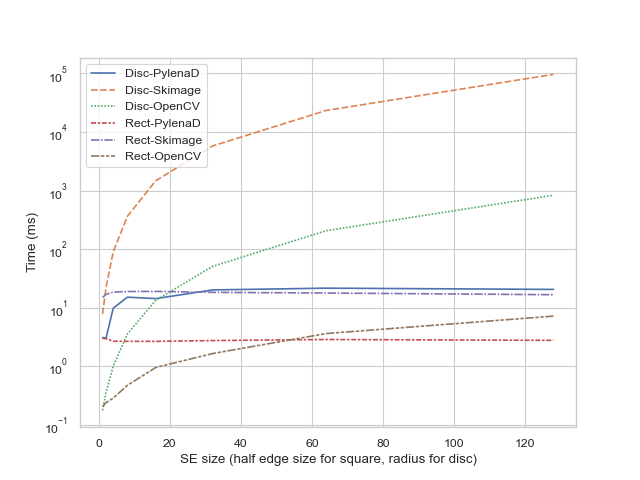
\includegraphics[width=3.8in]{../figures/bench_disc_rect_by_SE}
  %\caption{Benchmark: dilation of a 2D image (3128x3128 \eqmark 10Mpix) with a 2D square and a 2D disc. \FIXME{Légende image (noms, espace)}}
  \caption{Benchmark: dilation of a 2D image (\(3128 \times 3128\) \eqmark 10Mpix) with a 2D square and a 2D disc.}
  \label{fig:gen.bench.square.disc}
\end{figure}



In the case of a structuring element shaped as a disc (also in~\cref{fig:gen.bench.square.disc}), we can observe that
the execution time raises exponentially for both Scikit-image and OpenCV whereas Pylene remains regular and steady fast.
These results show that Pylene's attempt to decompose each structuring element into periodic lines when possible may be
slightly slower for smaller structuring elements whereas it is much more regular and faster when the structuring element
start to be of a certain size.

%\FIXME{Rajouter arbre de décision de l'algorithme final qui tourne sur chaque bibliothèque avec note sur les méthodes de
%  décisions (statiques ou dynamique)}

\subsubsection{Limitations regarding static types in a dynamic world}

Being statically typed (at language level) has its advantages (performance, optimization) but also has sever drawbacks,
especially when interfacing with dynamic languages such as Python. Indeed, being statically typed in a dynamic world
disqualify the library from being able to select, for instance, a new, custom structuring element, when performing a
dilation. As a matter of fact, all the supported structuring elements must be listed in advance and code must be
compiled for each supported type. This induces a strong inertia when the practitioner wants to try out new things not
yet supported by the library. This also defeats the initial purpose of being generic. Indeed, one would expect a generic
library to work with any type and not just a specified set of pre-compiled types. Being able to breakthrough this limit
is addressed more in-depth in~\cref{chap:static_dynamic_bridge}.


\subsection{Summary}

To conclude, a generic algorithm will not be faster after it is first written, but will provide acceptable performance
for most cases. However, a generic algorithm provide opportunities for the implementer to take advantage of some
properties from input types in order to be faster. The main advantage is that once those optimization opportunities are
written once, they are available for every input types (that match the property). Genericity enables code dispatching
very easily based on type property which may induce almost no runtime overhead, depending on which generic strategy was
chosen in the library.


\section{Genericity within programming languages}
\label{sec:gen.genericity.within.programming.languages}

Genericity is a more than 45 years old notion. It was first introduced alongside the CLU language in 1974 by Barbara
Liskov and her students~\parencite{liskov.1993.cluart}. The language offered many features such as data encapsulation,
iterators and especially \emph{parametrized modules}. A module in CLU is represented by a \emph{cluster}. A
\emph{cluster} is a programming unit grouping a data structure and its related operations. In modern programming, we
would call it a class where the data structure correspond to the member variables and the operations correspond to the
member functions (or methods). In CLU, the clusters can be parametrized which is a way to introduce the notion of
parametric polymorphism. Indeed, clusters offered the ability to define a generic data structure and its functions whose
behavior will not change whatever type the cluster is parametrized with. At first, type-safety was enforced at runtime
in CLU. Later, \emph{where clauses} were introduced to specify specific requirements over cluster type parameters. This
had the consequence of allowing only the operations required in the where clause to be used in the cluster
implementation code. This enables proper compile-type checks, type-safety and the compilation into a simple native and
optimized code by the compiler. The following code illustrates how to create a cluster (or class) named \emph{vector},
declaring a set of member functions and requiring a specific behavior (operator \(=\) and \(<\)) from its underlying
stored elements:

\begin{minted}{cobol}
  vector = cluster [T: type] is
    create, size, contains, sort, remove, push_back
  where
    T has equal: prototype(T, T) return (bool)
    T has less: prototype(T, T) return (bool)
\end{minted}

When implementing the member functions declared for \texttt{vector}, the only valid operations that can be performed on
a value of type \texttt{T} are \texttt{equal} (\(=\) for comparison) and \texttt{less} (\(<\) for ordering). In CLU the
actual instantiation of the parameter (here \texttt{T}) is done at runtime. Indeed, each type is represented by a
descriptor, even a parametrized type parameter. At runtime, a concrete type is used to instantiate the cluster. To
achieve this, the placeholder type descriptor is replaced by the one of the actual concrete type at this moment. The
instantiation can then be considered dynamic which differs from the C++ compilation model where the template
instantiation is considered static (\ie done at compile-time). The \pros and \cons of this approach are discussed
in~\parencite{atkinson.1978.cluimpl} which essentially are the resulting binary code size due to combinatorial explosion
combined with optimized code generation versus small, flexible and slower binary.

Later on came the Ada programming language whose conception work started in 1977 and first version was released in 1980.
It was first standardized in 1983~\parencite{ansi.1983.ada} in the United States by the American National Standards
Institute (ANSI) before being Internationally standardized by the International Organization for Standardization (ISO)
in 1987~\parencite{iso.1987.ada}. From this point on, the Ada language released a new version in
1995~\parencite{iso.1995.ada, iso.1995.ada.corr}, then the standard committee published an Amendment in
2007~\parencite{iso.1995.ada.amend} which is often referred as Ada 2005. Finally, a new version of the language was
published in 2012~\parencite{iso.2012.ada,iso.2012.ada.corr}. What interest us in the Ada language is the fact that the
language features \emph{generics} since it was first designed in 1977--1980 which \emph{ten years} before Musser and
Stepanov published their first work about genericity in 1988~\parencite{musser.1988.generic}. Indeed, it took around 20
years for the fist Standard Template Library (STL) will then be standardized in the C++ programming language in
C++98~\parencite{iso.1998.cpp}. It then took almost 10 more years for an STL to land into the Ada programming language
in the 2007 Amendment for Ada 2005.

In the Ada programming language, it is possible to mark a package or a procedure as generic with the \texttt{generic}
keyword. The developer then lists the parametrized parameter the package and/or the function requires to be implemented.
The following code demonstrates how this feature work by implementing a function replacing the first argument by a new
value and returning its previous value (also known as exchange).

\begin{minted}{Ada}
generic
  type T is private;
function exchange (x : in out T; v : in T) return T is
  tmp : T;
begin
  tmp := x;
  x   := v;
  return tmp;
end exchange;
\end{minted}

In Ada, generic packages and routines (procedures, functions) must be instantiated explicitly: the compiler cannot infer
the parametrized type at compile time from the context of use (whereas a C++ compiler can). Thus, the following three
lines must be written explicitly for the compiler to generate the binary code of the above function:
\begin{minted}{ada}
  function int_exchange is new exchange (Integer);
  function float_exchange is new exchange (Float);
  function str_exchange is new exchange (String);
\end{minted}

In Ada, this model enables the possibility of sharing a generic across several compilation units since its compilation is
independent of its use whereas in C++, until C++20 the sharing model consists in copy-pasting the whole source code
(and transitive recursive dependencies) each time a generic (a template) code is compiled. C++20 (standardized in 2020,
42 years after C++98) bring a solution to this issue by standardizing C++ modules. However, this feature is out of scope
of this study and will not be discussed in this thesis.

Also, Ada support syntactic constraints on parameters similar to the CLU language. It is translated into a \texttt{with}
clause listing the constraints on the parameter(s). The following code shows how to implement such a constrained generic
function by using the mathematical maximum operator as an example:

\begin{minted}{ada}
generic
  type T is private;
  with function "<" (x, y: T) return Boolean is <>;
function maximum (x, y : in T) return T is
  tmp : T;
begin
  if x < y then
    return x;
  else
    return y;
  end if;
end maximum;
\end{minted}

Let us not forget to instantiate the constrained generic function for integers:

\begin{minted}{ada}
  function int_maximum is new maximum (Integer);
\end{minted}

This idea of constrained generic is 30 years old and has only made his way very recently (2020) in the C++ programming
language under the feature name of \emph{concepts}.

Now that we have introduced where generic programming is coming from, let us focus on the C++ programming language and
how it has made his way into the language along the last 30 years, as well as along the years to come.

\subsection{Genericity in pre C++11}
\label{sec:precpp11}

Before C++11~\parencite{iso.2011.cpp} came out the genericity facilities offered by the C++ programming language were
already Turing-complete~\parencite{veldhuizen.2003.c++templates}. However, it was lacking a certain amount of features
the language now have that made writing generic code a real challenge at that time. For instance, when writing code with
a variable number of types (nowadays designated as variadic templates) one had to write the generic code for each and
every number of type supported. This meant that to implement \texttt{std::tuple}, one had to copy the implementation for
every number of type supported by \texttt{std::tuple}. This limitation defeated the very first principle and motivation
of generic programming which is to write \emph{less} Code. To compensate, library implementers used tricks with macro
not to have to rewrite code which made the initial code even harder to understand for outsiders.


\subsubsection{Functions on types (or traits)}

The very first feature every developer writing metaprogramming C++ code has used is called \emph{type-traits}. Those
\emph{traits} are a way to mutate a type depending on the way a template declared on a data structure is resolved.
Indeed, in C++ the instantiation of a template depends on the context, which means the compiler is required to build a
set of possible way to resolve a template instantiation and in order to determine the best match to resolve the
instantiation. This mechanism is well known and documented in the C++ standard, it can then be used (and abused) to do a
great number of things. Among all the traits that exist (a lot of them have been standardized in C++11, 2011, in the
header \texttt{<type\_traits>}), some in particular are used in every codebase: \texttt{remove\_const},
\texttt{remove\_volatile} and \texttt{remove\_reference}. Let us see how they are implemented:

\begin{minted}{C++}
  template<class T> struct remove_const                { using type = T; };
  template<class T> struct remove_const<const T>       { using type = T; };

  template<class T> struct remove_volatile             { using type = T; };
  template<class T> struct remove_volatile<volatile T> { using type = T; };

  template<class T> struct remove_reference            { using type = T; };
  template<class T> struct remove_reference<T &>       { using type = T; };
  template<class T> struct remove_reference<T &&>      { using type = T; };
\end{minted}

For \texttt{remove\_const}, first is defined the structure whose underlying alias \texttt{type} points to the passed
template parameter \texttt{T}. Then we define a template specialization whose matching parameters are all \texttt{T}
parameters that are \texttt{const}. The defined underlying alias \texttt{type} for this specialization then is
\texttt{T} without the qualifying \texttt{const}. This way, there are two possibilities when calling this \texttt{trait}
(or metafunction): either the passed parameter is not \texttt{const} which means it will be forwarded as-is to the
underlying alias \texttt{type} or the passed parameter is \texttt{const} which means the underlying alias \texttt{type}
will be defined by dropping the \texttt{const-qualifier} off of the passed parameter type. For instance:

\begin{minted}{C++}
  using T1 = remove_const<double>::type // T1 is double
  using T2 = remove_const<const double>::type // T2 is double too, const-qualifier is dropped
\end{minted}

This language construct is very useful when developing generic libraries because it enables performing ``functions'' on
types, and even chain them. It is also possible to perform checks to extract information about those types. We can
easily write an \texttt{is\_const} metafunction if we need it.

In image processing in particular, the usage of traits in the generic library Milena was very useful to achieve standard
ways to compute very useful types from other complex type. From the image processing definition of an image type, we can
already see a number of traits that a generic library would want to provide. Indeed, it would be useful to be able to
extract the type of the domain (box2d, box3d, etc.), the type of the point (point2d, point3d, \ldots), the underlying
value type (uint8, rgb8, etc.) and so on. We can also already see emerging consistency issues between those types.
Indeed, a box3d domain would not accept access via a point2D. It would instead require a point3d. All those issues will
be addressed later in the~\cref{chap:image.algorithms.taxonomy}. However, we can already give here minimal working
example as to how type traits are especially useful in a generic image processing library. First let us define some
minimal data structures:

\begin{minted}{C++}
  struct point2d {int x, y; };
  string rgb8 { uint8_t r, g, b; };
  struct box2d {
    using value_type = point2D;
    // ...
  };
  struct image2d {
    using domain_type = box2d;
    using point_type  = point2d;
    using value_type  = rgb8;
    // ...
  };
\end{minted}

Now we would want to implement \texttt{traits} to extract type information from those structures. Here is how we do it
in a generic library:

\begin{minted}{C++}
  template <class T> struct domain_value_type { using type = typename T::value_type;  };
  template <class T> struct image_point_type  { using type = typename T::point_type;  };
  template <class T> struct image_value_type  { using type = typename T::value_type;  };
  template <class T> struct image_domain_type { using type = typename T::domain_type; };
\end{minted}

These traits extract information about types in a generic way and can be used in any algorithm taking an image as a
template parameter. For instance, here is how an image processing algorithm (trivially extracting the max value) would b
e written:

\begin{minted}{C++}
template <class Ima>
typename image_value_type<Ima>::type // usage of trait
min_value(const Ima& ima) {
  using value_t = typename image_value_type<Ima>::type; // usage of trait
  auto min = std::numeric_limits<value_t>::max();
  for(auto v : ima.values()) {
    auto min = std::min(min, v);
  }
  return min;
}
\end{minted}

\subsubsection{SFINAE: Substitution-Failure-Is-Not-An-Error}
\label{subsec:sfinae}

Additionally, another feature related to metaprogramming  allowed the developer to design generic libraries: the
SFINAE~\parencite{vandevoorde.2002.c++} (substitution-failure-is-not-an-error) technique that leads to the
popularization of the usage of the \texttt{std::enable\_if} metaprogramming construct. The SFINAE technique relies on a
feature of the C++ programming language. Indeed, when standardizing how the compiler should resolve and select function
overloads, in a templated context, the standard committee chose to have the following behavior: ``when substituting the
explicitly specified or deduced type for the template parameter fails, the specialization (function overload candidate)
is discarded from the overload set (of matching functions) instead of causing an error''.

This feature allows writing code that seem to be ill-formed, for instance in a function, trying to access a class member
type, variable or function that does not exist should be ill-formed. However, because it happens in a templated context
during the instantiation resolution, when the compiler tries to instantiate a function template with a parametrized
type, the compiler will just discard the function from the overload resolution set at call-site instead of throwing a
hard error. An error can occur only when the compiler tried all the overload it knows in the overload set and still
could not find an overload that was not ill-formed. If this happens, the compiler will then proceed to list all the
overloads it tried, to list all the template substitution it tried and finally to list why it failed. This mechanism is
the very reason of the unpopularity of this technique because it leads to situation where the compiler can output
\emph{several Mos} of error message for one single file. Error messages become incomprehensible very fast and programs
are hard to debug because everything happens at compile-time. But still, it was the only technique we had to perform any
kind of detections on types at compile time to require some any given constraints on them.

For instance, here is some real-world example extracted from generic image processing code that allows implementing the
\emph{fill} algorithm in two very different ways depending on how behaves the input image type. First we need to write
the detector which is a structure whose templated context will be ill-formed during template instantiation. This
detector will inherit either \texttt{std::true\_type} or \texttt{false\_type} depending on whether the detection is
successful or not:

\begin{minted}{C++}
  // Step 1 write detector
  template <class Ima, class = void>
  struct is_image_with_lut : std::false_type {};

  template <class Ima>
  struct is_image_with_lut<Ima,
     typename Ima::lut_type // constraint over the existence of the lut_type field
  > : std::true_type {};
\end{minted}

Now let us introduce a new image type for the sake of this example:

\begin{minted}{C++}
  struct image2d_lut : image2d {
    using lut_type = std::array<uint8_t, 256>;
    using value_type = uint8_t:
    lut_type& get_lut();
  };
  template <class Ima>
  struct image_lut_type {
    using type = typename Ima::lut_type;
  }
\end{minted}

The next step is to implement the \texttt{enable\_if} facility. This is included in the C++ STL starting from C++11 and
onward:

\begin{minted}{C++}
  template<bool B, class = void>
  struct enable_if {};

  template<class T>
  struct enable_if<true, T> {
    using type = T;
  };
\end{minted}

Now we are all set to use all those construct to dispatch our algorithms from call-site depending on our input image
type:

\begin{minted}{C++}
  // Overload #1 : with lut
  template <class Ima,
  void fill(Ima& ima, typename image_value_type<Ima>::type val,
            typename enable_if<is_image_with_lut<Ima>::type::value, void*>::type = 0)
  { // Image with lut
    using lut_t = typename image_lut_type<Ima>::type;
    using value_t = typename image_value_type<Ima>::type;
    lut_t& lut = ima.get_lut();
    for(value_t& v : lut)
      v = val;
  }

  // Overload #2 : without lut
  template <class Ima,
  void fill(Ima& ima, typename image_value_type<Ima>::type val,
            typename enable_if<not is_image_with_lut<Ima>::type::value, void*>::type = 0)
  { // Image without lut
    using value_t = typename image_value_type<Ima>::type;
    for(value_t& v : ima.values())
      v = val;
  }
\end{minted}

Finally, let us give some call-site example to finish illustrating our point:

\begin{minted}{C++}
  image2d_lut ima1;
  image2d ima2;

  fill(ima1, 0);   // will dispatch over overload #1
  fill(ima2, 255); // will dispatch over overload #2
\end{minted}
Here, no hard error occur. Both overload are dispatched according to the constraint built with the SFINAE construct. Now
we can talk about \emph{constrained genericity} in C++. If we had an algorithm returning a value instead of performing
an in-place computation, we would have been able to write the code with the SFINAE construct in the return-type instead
of having it in the templates parameters. However, that is not the case here.


\subsubsection{CRTP: Curiously Recurring Template Pattern}
\label{subsec:crtp}

Another features that precede C++11 and was available in C++98~\parencite{iso.1998.cpp} and
C++03~\parencite{iso.2003.cpp} is the curiously recurring template pattern (CRTP) introduced in 1996 by
Coplien~\parencite{coplien.1996.crtp}. This programming technique allows a base class (in its specific code) to be aware
of its derived class at compile type. We made extensive use of this pattern in the past to design a new paradigm,
SCOOP~\parencite{burrus.2003.mpool, geraud.2006.scoop-pres, geraud.2008.mpool, levillain.2011.phd} which combined
multiple inheritance (via CRTP) and concept checking (via
Boost.Concept~\parencite{siek.2000.concept,boost.2006.concepts}) to implement a solution to provide a library with
constrained genericity in C++ for the image processing area. The Scoop paradigm relied on the fact that multiple
(especially diamond) inheritance did not pose much of an issue as long as there was no member variable involved. This
way, one could consider a class hierarchy as a hierarchy of constraint indeed. Using CRTP, it was possible to find back,
inside constraining classes, what was the concrete leaf class of the hierarchy in order to check whether its
implementation satisfied the constraints or not. For instance, let us assume that we have a concrete class
\texttt{image2d} inheriting from a constraining class \texttt{Image}. Let us now see how one would use the SCOOP
paradigm to implement it. First we need to implement the satellite constraints around the image type which are related
to the underlying point and domain of the image.

\begin{minted}{C++}
  template <class P>
  struct Point { // concept checking class
    int (P::*m_ptr1) const = & P::dim;
  };

  struct point2d : Point<point2d> { // CRTP
    int x, y;
    int dim() const { return 2; }
  };

  template <class D>
  struct Domain { // concept checking class
    using value_type = typename D::value_type;
    // ...
  };

  struct box2d : Domain<box2d> { // CRTP
    using value_type = point2d;
    // ...
  };
\end{minted}

For the sake of brevity, we are omitting the implementation of domain functions related to iterating over all the points
of the domain. With those concepts defined, we can now dig into how we would implement an image class with the SCOOP
paradigm.

\begin{minted}{C++}

  template <class I>
  struct Image { // concept checking class
    using value_type = typename I::value_type;
    using point_type = Point<typename I::point_type>;
    using domain_type = Domain<typename I::domain_type>;

    const domain_type& (I::*m_ptr1)() const = & I::domain;
    // ...
  };

  struct image2d : Image<image2d> { // CRTP
    using value_type = uint8_t;
    using point_type = point2d;
    using domain_type = box2d;

    // ... ctors ...

    const domain_type& domain() const {
      return m_dom;
    }
  private:
    domain_type m_dom;
  };
\end{minted}

Each time a leaf class in the hierarchy inherit from a base class, the concepts are checked. The syntax is not really
intuitive, especially writing the function pointers to check that their prototype is confirming a certain behavior, but
it was all what was available at that time. To be completely exhaustive, the library implementing this paradigm, Milena
featured another powerful tool which allows one to require only concept class into input data for algorithms. Inside the
algorithm it was then possible to get back the concrete class and use it as if it was originally passed as an argument.
To do so, it was needed to add a member field to the concept class named \texttt{exact\_t} that kept track of the leaf
class into the concept checking class.

\begin{minted}{C++}
  template <class I>
  class Image {
    // ...
    using exact_t = I;
  };
\end{minted}

Then a simple cast routine would do the trick inside the algorithm:

\begin{minted}{C++}
  #define EXACT(Ima) \
    typename Ima::exact_t

  template <class Ima> // mutable routine
  EXACT(Ima)& exact(Ima& ima) { return static_cast<EXACT(Ima)&>(ima); }

  template <class Ima> // const routine
  const EXACT(Ima)& exact(const Ima& ima) { return static_cast<const EXACT(Ima)&>(ima); }
\end{minted}

This way, in image processing algorithms, the implementer would only need to write minimal code for it to work out of
the box:

\begin{minted}{C++}
  template <class I>
  void fill(Image<I>& ima, typename image_value_type<Ima>::type val) {
    EXACT(Ima)& ima_ = exact(ima);

    // use the concrete underlying image ima_ and val
  }
\end{minted}

This constrained genericity would be totally transparent as shown with the following code that just works out of the
box, thanks to the SCOOP paradigm and its inheritance strategy to constrain classes.
\begin{minted}{C++}
  image2d ima = /* ... */;
  uint8_t val = 0;
  fill(ima, val);
\end{minted}

By extension, this work on Milena was integrated in the image processing platform
Olena~\parencite{olena.2000.www,geraud.2012.hdr}. This platform centralizes the work that was done around this field of
research for a long time~\parencite{geraud.2000.icpr,duretlutz.2000.olena,darbon.2002.ismm,darbon.2004.ecoopphd}. More
details can be found about SCOOP, and notably how it enables property based programming (augmentation of types via
properties) in the work of
\citeauthor{levillain.2011.phd}~\parencite{levillain.2011.phd,levillain.2009.ismm,levillain.2010.icip,levillain.2010.wadgmm,levillain.2011.gretsi,levillain.2011.phd,levillain.2012.wadgmm-lncs,levillain.2014.ciarp}.

Those approaches have the advantage of being really flexible and to be able to perform the concept checking work that we
wanted to have, be it to constrain implementation or to dispatch to the correct overloaded algorithms depending on
specific properties. The disadvantages come in the form of an increased complexity of the design hierarchy of
implemented types as they must inherit concepts via CRTP and conform to specific constrains. Also, all the
implementation is visible as all the code is generic (template) and all the implementation details are leaked to the
user code. For an image processing library which can use several dependencies (for instance, a library that read images
from disc from multiple image formats), this is a huge drawback.

With the release of new C++ standards in 2011~\parencite{iso.2011.cpp}, then 2014~\parencite{iso.2014.cpp},
2017~\parencite{iso.2017.cpp} where template metaprogramming facilities were greatly improved, it was necessary to
review once more this design to improve the design in order to achieve genericity, performance and ease of use. This is
the birth of a new library, Pylene~\parencite{carlinet.2018.pylena}. In the end, it was C++20~\parencite{iso.2011.cpp}
that marked the shift wanted by
Stepanov~\parencite{musser.1988.generic,musser.1994.algorithm,dehnert.1998.fundamentals,stepanov.2009.elements} and
Stroustrup~\parencite{stroustrup.1995.design,stroustrup.1999.hot,stroustrup.2003.concepts,stroustrup.2007.hopl} for
years with the coming of Concepts, and all the new possibilities it brings to the programmer.

\subsection{Genericity in post C++11 (C++20 and Concepts)}
\label{sec:postcpp11}

\begin{figure}[htbp]
  \centering
  \begin{minted}[linenos,xleftmargin=17pt,gobble=2,highlightlines={2,4,5}]{c++}
  template <Image Ima, ValueType Val>
    requires same<Ima::value_type, V>
  void fill(Ima ima, Val val) {
    for(Val v : ima)
      v = val;
  }
  \end{minted}

  \caption{Fill algorithm, generic implementation.}
  \label{code:gen.fill}
\end{figure}

Most of the algorithms are \emph{generic} by nature. What limits their genericity is the way they are implemented. This
statement is justified by the work achieved in the Standard Template Library (STL)~\parencite{dehnert.1998.fundamentals}
in C++ whose algorithms are implemented and designed in a way where they work with all the built-in collections (linked
list, vector, etc.). Let us take the example of the algorithm \texttt{fill(Collection c, Value v)} which set the same
value for all the element of a collection (see~\cref{code:gen.fill}). There are three main requirements here that are
not related to the underlying type of \emph{Collection}. First, we check (l.2~\cref{code:gen.fill}) that we are actually
filling the collection with the correct type of value. Indeed, it would not make sense, for instance, to assign an RGB
triplet color into a pixel from a grayscale image. Secondly, we need to be able to iterate over all the element of the
collection (l.4~\cref{code:gen.fill}). Finally, we need to be able to write a value into the collection
(l.5~\cref{code:gen.fill}). This requires the collection not to be read-only, or the collection's values not to be
yielded on-the-fly. This allows us to deduce what is called a \emph{concept}: a breakdown of all the requirement about
the behavior of our collection. When writing down what a \emph{concept} should require, one should always respect this
rule: \blockquote{\emph{It is not the types that define the concepts: it is the algorithms}}. Concepts in C++ are not
new and there have been a long work to introduce them that goes back from
2003~\parencite{seymour.2009.concepts,stroustrup.2003.concepts,sutton.2017.concepts} to finally appear in the 2020
standard~\parencite{voutilainen.2017.concepts} (referred as C++20~\parencite{iso.2011.cpp}). This allows us, as of
today, to write code leveraging this facility.

\subsubsection{Conceptification}
\label{subsec:conceptification}

C++ is a multi-paradigm language that enables the developer to write code that can be \emph{object oriented},
\emph{procedural}, \emph{functional} and \emph{generic}. However, there were limitations that were mostly due to the
backward compatibility constraint as well as the zero-cost abstraction principle. In particular the \emph{generic
  programming} paradigm is provided by the \emph{template metaprogramming} machinery which can be rather obscure and
error-prone. Furthermore, when the code is incorrect, due to the nature of templates (and the way they are specified) it
is extremely difficult for a compiler to provide a clear and useful error message. To solve this issue, a new facility
named \emph{concepts} was brought to the language. It enables the developer to constraint types: we say that the type
\emph{models} the \emph{concept(s)}. For instance, to compare two images, a function \emph{compare} would restrict its
input image types to the ones whose value type provides the \emph{comparison operator ==}. In spite of the history
behind the \emph{concept checking} facilities being very
turbulent~\parencite{seymour.2009.concepts,stroustrup.2003.concepts,sutton.2017.concepts}, it will finally appear in the
next standard~\parencite{voutilainen.2017.concepts} (C++20).

The C++ \emph{Standard Template Library} (STL) is a collection of algorithms and data structures that allow the
developer to code with generic facilities. For instance, there is a standard way to \emph{reduce} a collection of
elements: \texttt{std::accumulate} that is agnostic to the underlying collection type. The collection just needs to
provide a facility so that it can work. This facility is called \emph{iterator}. All STL algorithms behave this way: the
type is a template parameter, so it can be anything. What is important is how this type behaves. Some collection
requires you to define a \texttt{hash} functions (\texttt{std::map}), some requires you to set an \emph{order} on your
elements (\texttt{std::set}) etc. This emphasis the power of genericity. The most important point to remember here (and
explained very early in 1988~\parencite{musser.1988.generic}) is the answer to: \blockquote{\emph{What is a generic
    algorithm?}}. The answer is: \blockquote{\emph{An algorithm is generic when it is expressed in the most abstract way
    possible}}. Later, in his book~\parencite{stepanov.2009.elements}, Stepanov explained the design decision behind those
algorithms as well as an important notion born in the early 2000s: the concepts. The most important point about concepts
is that it constrains the behavior. Henceforth: \blockquote{\emph{It is not the types that define the concepts: it is
    the algorithms}}. The \emph{Image Processing} and \emph{Computer Vision} fields are facing this issue because there are
a lot of algorithms, a lot of different kinds of images and a lot of different kinds of requirements/properties for
those algorithms to work. In fact, when analyzing the algorithms, you can always extract those requirements in the form
of one or several \emph{concepts}. This section is a preface to the image taxonomy which will be seen more in-depth
in~\cref{chap:image.algorithms.taxonomy}.

Image processing algorithms, similarly, are \emph{generic} by
nature~\parencite{ritter.1990.cvgi,geraud.2000.icpr,darbon.2002.ismm,levillain.2010.icip,levillain.2014.ciarp}. When
writing an image processing algorithm, there is always a way to express it with a high level of genericity. For
instance, if it is possible to write a morphological dilation in a way that does not care about the underlying value
type, the domain nor the structuring element specificities. The most abstract way to write a dilation is shown
in~\cref{code:gen.dilate}.

\begin{figure}[htbp]
  \centering
  \begin{minted}[linenos,xleftmargin=17pt,gobble=2]{C++}
  template <Image I, WritableImage O,
              StructuringElement SE>
  void dilation(I input, O output, SE se) {
    assert(input.domain() == output.domain());
    for(auto pnt : input.points()) {
      output(p) = input(p)
      for (nx : se(p))
        output(p) = max(input(nx), output(p))
    }
  }
  \end{minted}
  \caption{Dilation algorithm, generic implementation.}
  \label{code:gen.dilate}
\end{figure}

This implementation introduces three concepts at line 1: \emph{Image}, \emph{WritableImage} and
\emph{StructuringElement}. Following the behavior of each one of them into the algorithm, we can deduce a list of
requirements for each one of them.

\paragraph{Image} It is the most basic representation of what an image should be. An image should (a) provide a way to
access its domain (l.3~\cref{code:gen.dilate}) and (b) a way to iterate over its points (l.4~\cref{code:gen.dilate}).
This then allows us later to (c) access to the value returned by the image at this point (l.5~\cref{code:gen.dilate}).
To this point the value is only accessed in read-only. We can then write the following two concepts:
\begin{minted}{C++}
  template <typename I>
  concept Image = requires {
    typename I::point_range;            // needed for a
    typename I::point_type;             // needed for b
    typename I::value_type;             // needed for b
  } && ForwardRange<I::point_range>     // needed for a
  && requires (I ima, I::point_type pnt) {
    { ima.points() } -> I::point_range; // a
    { ima(pnt) }     -> I::value_type;  // b
  };
\end{minted}
In reality, more boilerplate code is needed to ensure, for instance that there is no type mismatch between the image's
\texttt{point\_type} and the \texttt{point\_range}'s value type. For the sake of brevity this boilerplate code is
omitted here.

\paragraph{WritableImage} It is a more specific concept based on the previous \emph{Image} concept. It requires that the
image's value can be (d) accessed to be modified: the user should be able to write into the image's value accessed by a
specific point (l.6~\cref{code:gen.dilate}). We can then write the following two concepts:
\begin{minted}{C++}
  template <typename WI>
  concept WritableImage = Image<WI>
  && requires (WI wima, I::point_type pnt,
                I::value_type val) {
    { wima(pnt) = val };                // d
  };
\end{minted}

\paragraph{StructuringElement} It is an additional input to the image defining the window around each point that will be
considered during the dilation (also called the neighborhood). A structuring element should just provide a list of point
when input with one (e). From this behavior we can deduce the following concept:
\begin{minted}{C++}
  template <typename SE, typename I>
  concept StructuringElement = Image<I>
  && requires (SE se,I::point_type pnt) {
    { se(pnt) } -> I::point_range;      // e
  }
\end{minted}

This new notion of concept is very important because it decorrelate the requirements on behavior required inside
algorithms from the way the data structures are designed. One wan always wrap a specific data structure so that it can
behave properly into an algorithm, without needing to rewrite that algorithm.

\subsubsection{Simplifying code}
\label{subsec:simplifying}

The main advantage brought by using modern C++ as the implementation language for an image processing library is to be
able to leverage what is called metaprogramming. Metaprogramming is a way to tell the compiler to make decision about
which type, which code to generate. These decisions, made at compile time, and then absent from the resulting binary:
only the fast and optimized code remains. This brings a new distinction between the static world (what is decided at
compile time) and the dynamic world (what is decided at runtime). The more is decided at compile time the smaller,
faster the binary will because there is work less to do at runtime. By following this principle, one can think of some
properties that are known ahead of time (at compilation) when writing one's image processing algorithm. For instance,
when considering the example of the dilation whose code is shown in~\cref{code:gen.dilate}, we can see that the property
about the decomposability of the structuring element is linked to the type. This means that when the structuring
element's type is of a disc, or a square, the compiler will know at compile time that it is decomposable. To tell the
compiler to take advantage of a property at compile time, C++ has a language construct named \emph{if-constexpr}. The
resulting code then becomes:

\begin{minted}[highlightlines=3]{c++}
  template <Image Img, StructuringElement SE>
  auto dilate(Img img, SE se) {
    if constexpr (se.is_decomposable()) {
      lst_small_se = se.decompose();
      for (auto small_se : lst_small_se)
        img = dilate(img, small_se) // Recursive call
      return img;
    } else if (is_pediodic_line(se))
      return fast_dilate1d(img, se) // Van Herk's algorithm;
    else
      return dilate_normal(img, se) // Classic algorithm;
  }
\end{minted}

There are other ways to achieve the same result with different language constructs in C++. There are two ``legacy''
language constructs which are tag dispatching (or overload) and SFINAE. With the release of C++17 came a new language
construct presented above: \emph{if-constexpr}. Finally, with C++20, it will be possible to use concepts to achieve the
same result. To achieve the same result as above with tag dispatching, one would need to write the following code:

\begin{minted}[highlightlines={1-2,7,14}]{c++}
  struct SE_decomp {};
  struct SE_no_decomp {};

  template <Image Img, StructuringElement SE>
  auto dilate(Img img, SE se) {
    // either SE_decompo or SE_no_decomp
    return dilate_(img, se, typename SE::decomposable());
  }

  auto dilate_(Img img, SE se, SE_decomp) {
    lst_small_se = se.decompose();
    for (auto small_se : lst_small_se)
      // Recursive call
      img = dilate(img, small_se, SE_no_decomp)
    return img;
  }
  auto dilate_(Img img, SE se, SE_no_decomp) {
    if (is_pediodic_line(se))
      return fast_dilate1d(img, se) // Van Herk's algorithm;
    else
      return dilate_normal(img, se) // Classic algorithm;
  }
\end{minted}

To achieve the same result with SFINAE, one would need to write the following code:

\begin{minted}[highlightlines={5-6,14,23}]{c++}
  // SFINAE helper
  template <typename SE, typename = void>
  struct is_decomposable : std::false_type {};
  template <typename SE>
  struct is_decomposable<SE,
    // Check wether the type provides the decompose() method
    std::void_t<decltype(std::declval<SE>().decompose())>
  > : std::true_type {};
  template <typename SE>
  constexpr bool is_decomposable_v =
                  is_decomposable<SE>::value;

  template <Image Img, StructuringElement SE,
    typename = std::enable_if_t<is_decomposable_v<SE>>>
  auto dilate(Img img, SE se) {
    lst_small_se = se.decompose();
    for (auto small_se : lst_small_se)
      img = dilate(img, small_se) // Recursive call
    return img;
  }

  template <Image Img, StructuringElement SE,
    typename = std::enable_if_t<not is_decomposable_v<SE>>>
  auto dilate(Img img, SE se) {
    if (is_pediodic_line(se))
      return fast_dilate1d(img, se) // Van Herk's algorithm;
    else
      return dilate_normal(img, se) // Classic algorithm;
  }
\end{minted}

Comparing those two last ways of writing static code to the first one comes to an obvious conclusion: the
\emph{if-constexpr} facility is much more readable and maintainable than the two legacy ways of doing it. Finally, there
is still another way to handle the issue, and it is with C++20's concepts. The following code demonstrates how to
leverage this language construct:

\begin{minted}[highlightlines={1-4,15}]{c++}
  template <typename SE>
  concept SE_decomposable = requires (SE se) {
    se.decompose(); // this method must exist
  };

  template <typename Img, typename SE>
  auto dilate(Img img, SE se) {
   if (is_pediodic_line(se))
      return fast_dilate1d(img, se) // Van Herk's algorithm;
    else
      return dilate_normal(img, se) // Classic algorithm;
  }

  template <typename Img, typename SE>
    requires SE_decomposable<SE>
  auto dilate(Img img, SE se) {
    lst_small_se = se.decompose();
    for (auto small_se : lst_small_se)
      img = dilate(img, small_se) // Recursive call
    return img;
  }
\end{minted}
A best-match mechanic~\parencite{dosries.2066.specifying.proc} operates under the hood to select the function overload
whose concept is the most specialized when possible. The best-match is very interesting to us as it removes completely
the need to have mutually exclusive conditions which were required with the SFINAE technique and could result in
explosive complexity with the growing number of \emph{and}/\emph{or} clauses. The best-match mechanic, works on top of
another widely used machinery in C++: the function overload set. For a specific function call, all the functions
overloads will be considered in the overload set. Then, to select the correct one, they will be sorted according to the
best-match procedure. Finally, if there is still two overloads that have the same priority, the compiler will raise a
hard error stating that there is an ambiguity it cannot solve on its own. As a matter of fact, adding one more function
to the overload set is enough to have it selected when it matches without modifying the already existing functions. One
could have added, in our example, an overload for structuring element whose shape is a periodic line, assuming that this
is a property that we can detect at compile-time.

\section{C++ templates in a dynamic world}
\label{sec:template.dynworld}

There are two main categories of programming languages. First are the \emph{compiled} programming languages which
requires to feed the source code to a program (a compiler) that will output a binary. This binary will then produce the
desired output once the user execute it. Some well known languages of this category are C, C++, Ada, Fortran. Secondly
there are the interpreted programming language which requires to feed the source code to a program (an interpreter) that
will directly produce the output as is a binary was executed. Some well known languages of this category are Javascript,
Python, Matlab, Common Lisp. There is a third category that tries to combine the best of both world by compiling into
bytecode which is an optimized intermediate language that will then be interpreted into a virtual machine. The most
famous are indubitably Java and C\#. Both categories have advantages and drawbacks.

\paragraph{Compiled languages} They are still widely spread and used as of today. They present a working pipeline which
is very classic. First the programmer will write code, then the compiler will build a binary optimized for the target
machine and finally the programmer can execute his binary to produce a result. Usually the compilation step is slow
whereas executing the binary is fast. There is no additional step when it comes to the binary execution. This, however,
has the effect of having a poor portability. Indeed, my binary optimized to use fast and recent SIMD AVX-512
instructions will not work on an old x86 machine that does not support those instructions. When distributing our
program, multiple binaries must be produced for each supported CPU architectures. Furthermore, usually compiled
languages have very poor support of dynamic language features such as reflection, code evaluation or dynamic typing. It
tends to improve with time but solutions are limited to compile-time information or need to ship a JIT-compiler into the
final binary (such as cling~\parencite{vassilev.2012.cling} for C++) to generate new binary on-the-fly to be executed
right after. This has two drawbacks: slowness when the case of needing compilation is presented and increase in the
binary size.

\paragraph{Interpreted languages} They are also widely used, especially in the research area where a fast feedback loop
between prototyping and getting results is needed. The compilation time is very fast and allows a program to be almost
instantly executed. In fact, the compilation can be done just ahead of program execution not to compile unnecessary
code. However, the execution time will generally be slow. To the user it is invisible because both compilation step and
execution step are blurred together. Furthermore, most of the time a same interpreted program is executed once. Then the
programmer will modify it and continue its prototyping process. The real advantage of an interpreted language is the
portability. As it is the responsibility of the client to install the correct language interpreter (for the correct
version) before running the program from the source code, as long as an interpreter can be installed on a machine, the
program can then be run. This also drastically slow distributed package for programs as only source code must be
distributed instead of compiled binary. However, the source code is leaked with all the security implication this can
have. Finally, interpreted language usually have better memory management (built-in garbage collectors), are easier to
debug, have very rich support of dynamic typing, dynamic scoping, reflections facilities, on-the-fly evaluation from the
source code or even more like modifying the Abstract Syntax Tree (AST) resulting from the first compilation pass on
source code by the interpreter. This last one is implemented in Common Lisp in the name of macros. There are more to say
about interpreted languages, especially about those that are compiled into bytecode and tend to get the best of both
worlds without the drawbacks, but this thesis will not discuss this matter any further.

The main point to understand here is that our main interest is set on C++, a compiled language with slow compilation
time and very fast execution time. In C++ there are template metaprogramming to achieve genericity, but \emph{templates
  do not generate any binary code}. Why? Because when the compiler meet a templated type or a templated routine, it does
not know which type it will be instantiated with when it is used. Therefore, it can not calculate stuff like type size,
alignment, can not select which assembly instruction to select to do an addition or a division (fixed \vs floating
point arithmetic). This is why the compiler does not generate any binary code when it first meets templates. The code is
generated only it is used with a concrete and known type. This is a huge problem. Now, if a library implementer wants to
distribute his generic library, he must distribute source code and have  the user compile it. For a language like C++,
with no standard dependency management, it can be a massive turn off. Furthermore, it may not be reasonable for the user
to have C++ compiling facilities when the target client is embedded devices with limited storage space. Indeed, C++
intermediary compilation artifacts tend to use a lot of disk space before it is linked into a smaller binary. What
solution do we have then?

\paragraph{SWILENA~\parencite{beazley.1996.swig,olena.2000.www}} It is a Python bindings wrapper using Swig for the
Olena C++ generic library. This wrapper will enumerate all the common use cases and implement a binding for them. The
compiler will then generate binary code from the templated generic code for each use case enumerated in the wrapper.
This way, we have given access into the dynamic world (Python) to generic code (C++ template). But it is still limited
to the supported types. Each type a new combination of type needs to be supported from Python, it needs to be explicitly
declared and compiled in the wrapper. Other image processing libraries, such as VIGRA~\parencite{kothe.2011.generic},
chose this solution.

\paragraph{VCSN~\parencite{demaille.2013.vcsn}} It is a novel solution that essentially take the same base as SWILENA
but goes beyond the boundary to implement a handmade facility that do system compiler calls to compile and link needed
code on-the-fly when the binding does not exist. It then leverages the code hot loading feature to plug new dynamic
libraries (.dll on Windows and .so on Linux) into the wrapper to provide the user its needed bindings.

\paragraph{Cython~\parencite{behnel.2010.cython}} It attempts to solve the issue of the Python inherent language
slowness due to its interpreted nature by providing a facility able to transpile a Python program into a C program so
that a genuine C compiler (with extensions) is able to compile it and to link it against the Python/C API in order to
achieve an important performance gain at the cost of near zero knowledge of the complex Python/C API for the user. This
novel solution essentially bypass the work of a JIT compiler (that would be used by a programming language using
bytecode such as Java or C\#) and just offload it onto well known/proven solution: the machine's C compiler.

\paragraph{AutoWIG~\parencite{fernique.2018.autowig}, Cppyy~\parencite{wimtlplavrijsen.2016.cppyy} and
  Xeus-cling~\parencite{quantstack.2021.xeus-cling}} are all solutions aiming to generate automatically Python bindings
on-the-fly using different solutions. AutoWIG has in-house code based on LLVM/Clang to parse C++ code in order to
generate and compile a Swig Python binding using the Mako templating engine. Cppyy will generate Python bindings but can
also directly interpret C++ code from Python code thanks to being base on LLVM/Cling, a Clang-base C++ interpreter.
Finally, Xeus-cling is a Jupyter~\parencite{kluyver.2016.jupyter} kernel allowing to directly interpret C++ into a
Jupyter notebook. Like Cppyy, it is based on LLVM/Cling. Those three projects are very promising and improve greatly the
scope of possibilities for the future.


\section{Summary}

In this chapter we present the origin of generic programming, which goes as far as~\citedate[year]{musser.1988.generic}
and how it has evolved to be integrated in the Ada programming language and then the C++ programming language.
Afterwards, it has evolved even further with the notion of \emph{concept} which completes the toolbox required to be
able to fully make use of generic programming without resorting to obscure tweaks and tools.

This chapter explores the possibilities of achieving the notion of genericity from within a library. Indeed, there are
three techniques enabling the user to write a high level algorithm once that can run on every type. They are the
\emph{code duplication} approach, the \emph{generalization} approach and the \emph{inclusion and parametric
  polymorphism} approach. We present in~\cref{table:gen.approaches} the result of the comparison of these approaches with
regard to the features that we are interested in. We also discuss the limitations linked to the usage of those
approaches by comparing OpenCV, Scikit-Image and Pylene which make use of the four techniques at different level to
achieve different goals. Furthermore, we have identified limitations related to the underlying data type, the structure of the
domain, the optimizations and discuss the performances through a concrete benchmark presented
in~\cref{fig:gen.bench.square.disc}.

This chapter also explores how the notion of genericity is achieved with the programming languages. We retrace how Ada
implemented it and then how C++ permitted the expression of require-clauses (concept) as soon as C++98, even though it
was limited at that time. We explore how template metaprogramming techniques have been developed and have evolved,
alongside the C++ programming language itself, to finally reach a point in 2020 (C++20) where it is possible to write
concepts in C++.

Finally, this chapter presents the inherent limitation of C++ templates, which is that they remain in the static world
(compile time). Genericity (in the sense C++ template) does not exist in the final shipped binary to the user. The final
user, in its dynamic world (runtime) cannot use a generic (C++ code) tool. We discuss the different approaches possible
to bridge this gap between the static (compile-time) and dynamic (runtime) world.

The next chapter will make extensive use of Genericity to present the first contribution of this thesis: a taxonomy of
concepts related to Image processing.
